\documentclass{article}

\usepackage[spanish]{babel}
\usepackage[numbers,sort&compress]{natbib}
\usepackage[T1]{fontenc}
\usepackage[ansinew]{inputenc}
\usepackage{graphicx}
\usepackage{url}
\usepackage{caption}
\usepackage{subcaption}
\usepackage{float}


\title{Pr\'actica 4: Diagramas de Voronoi}
\author{Anahi Llano}
\begin{document}
\maketitle

\section{Introducci\'{o}n.}\label{into}

Se realiza la cuarta pr\'actica \cite{elisa} llamada diagramas de voronoi.

 \section{Objetivo.}\label{obj}

El objetivo fue realizar una examinaci\'on sistem\'atica entre el efecto del n\'umero de semillas y el tama\~no de la zona de distribuci\'on de las grietas que se forman en t\'erminos de la mayor distancia euclideana.


\section{Metodolog\'{i}a.}\label{met}

De acuerdo al c\'odigo mostrado en clase \citet{elisa1} se agreg\'o la funci\'on para determinar la distancia m\'axima, corriendo el c\'odigo varias veces variando el tama\~no de la celda as\'i como el n\'umero de semillas de esta, as\'i mismo se realiz\'o una comparaci\'on entre la distancia m\'axima en manhatthan y euclideana.

\section{Resultados y Discusi\'{o}n.}\label{res}

Una vez obtenido el c\'odigo\citep{ana} se hizo una variaci\'on para examinar la distancia m\'axima de la grieta, variando el tama\~no de la celda y las semillas de esta. 
El c\'odigo se corri\'o varias veces para celdas de 30x30, 50x50,y 80x80, as\'i mismo se vari\'o la cantidad de semillas para todos los tama\~nos tomando semillas de 3-6,5-20,30-50 para tener un an\'alisis m\'as completo.
Para las gr\'aficas se tom\'o en cuenta en el eje de las ``x''  la variaci\'on de las semillas y en el eje de las ``y''  la distancia m\'axima para cada n\'umero de semillas.


\begin{figure}[H]
       \centering
       \begin{subfigure}[b]{0.7\linewidth}
           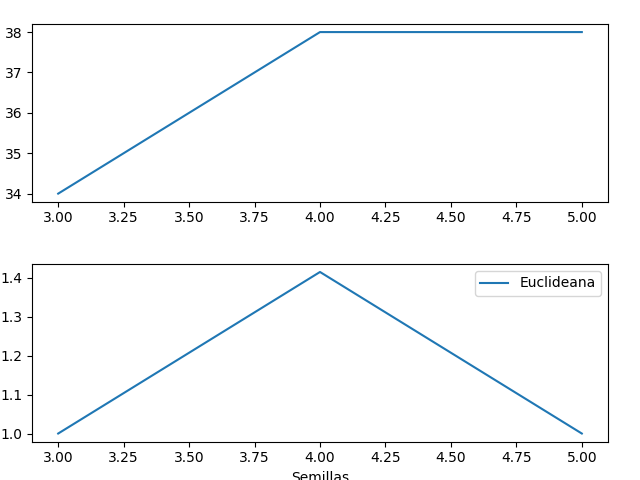
\includegraphics[width=\linewidth]{30x30.png}
           \caption{30x30}
           \label{fig:westminster_lateral}
        \end{subfigure}
        \begin{subfigure}[b]{0.7\linewidth}
            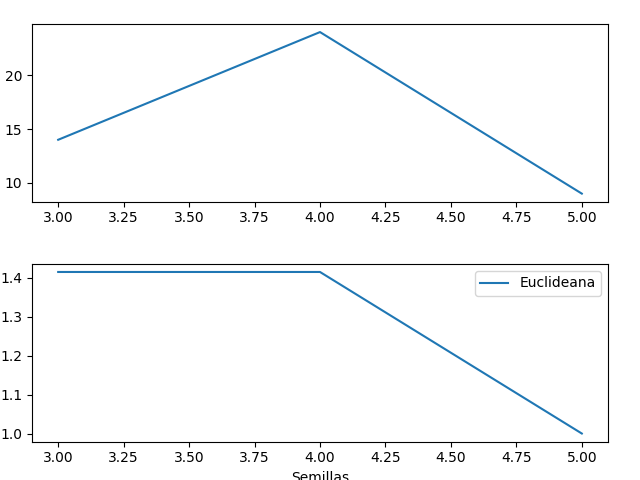
\includegraphics[width=\linewidth]{50x50.png}
            \caption{50x50}
            \label{fig:westminster_aerea}
        \end{subfigure}
        \begin{subfigure}[b]{0.7\linewidth}
           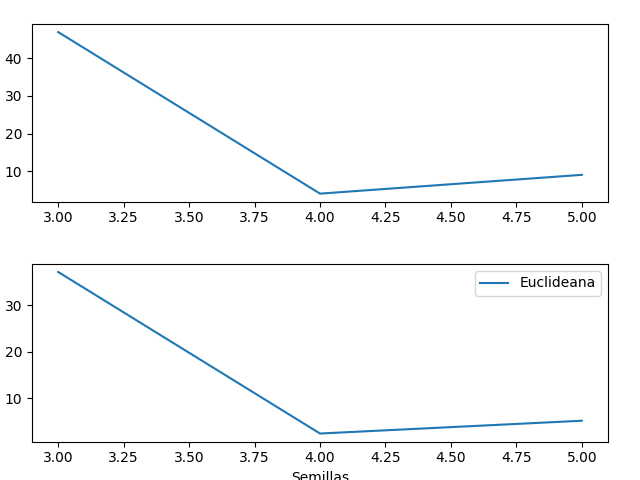
\includegraphics[width=\linewidth]{80x80.png}
           \caption{80x80}
           \label{fig:westminster_aerea}
        \end{subfigure}
        \caption{Variacion en semillas de 3-6}
        \label{f1}
\end{figure}

En la figura \ref{f1}  se puede observarla variaci\'on que se realiz\'o tomando tama\~nos de 30,50 y 80, as\'i como una cantidad reducida de semillas que va de 3-6. se puede observar la distancia m\'axima euclideana asi como la manhattan.
Cuando tenemos un tama\~no de 30x30 y utilizamos solo 4 semillas observamos que la distancia de la grieta aumenta, es mayor ah\'i en comparaci\'on de cuando tenemos 3 o 5 semillas, en cambio con un tama\~no de 80x80 la distancia m\'axima de la grieta es m\'as grande cuando tenemos 3 o 5 semillas a que cuando tenemos 4 en comparaci\'on de cuando el tama\~no de la celda es menor.

\begin{figure}[H]
       \centering
       \begin{subfigure}[b]{0.45\linewidth}
           
\includegraphics[width=\linewidth]{3semillas_3.png}
           \caption{30x30}
           \label{fig:westminster_lateral}
        \end{subfigure}
        \begin{subfigure}[b]{0.45\linewidth}
            
\includegraphics[width=\linewidth]{5semillas_5.png}
            \caption{50x50}
            \label{fig:westminster_aerea}
        \end{subfigure}
        \caption{Grieta en celdas de 3 y 5 semillas.}
        \label{f2}
\end{figure}

 As\'i mismo en la figura \ref{f2} se observa la diferencia en el tama\~no de la grieta cuando tenemos 3 a cuando tenemos 5 semillas. En una celda de 80x80.

\begin{figure}[H]
       \centering
       \begin{subfigure}[b]{0.7\linewidth}
           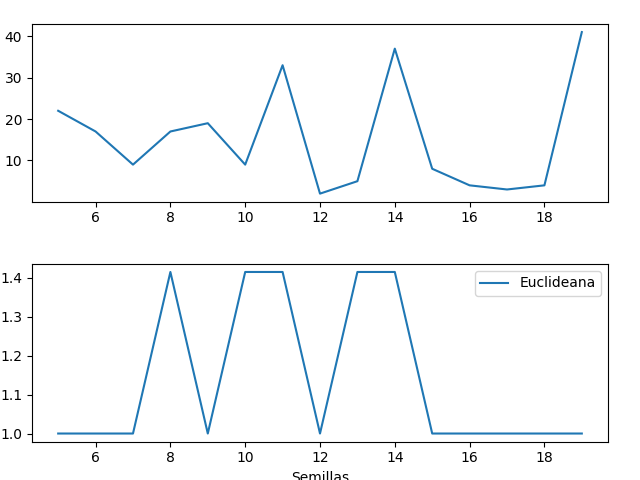
\includegraphics[width=\linewidth]{30x30-5-20.png}
           \caption{30x30}
           \label{fig:westminster_lateral}
        \end{subfigure}
        \begin{subfigure}[b]{0.7\linewidth}
            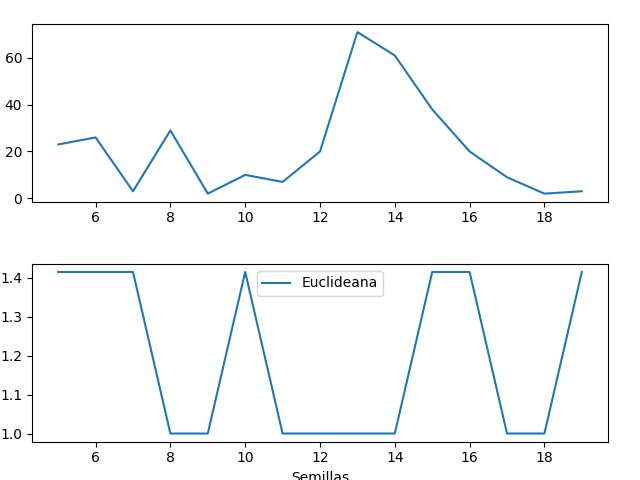
\includegraphics[width=\linewidth]{50x505-20.png}
            \caption{50x50}
            \label{fig:westminster_aerea}
        \end{subfigure}
        \begin{subfigure}[b]{0.7\linewidth}
           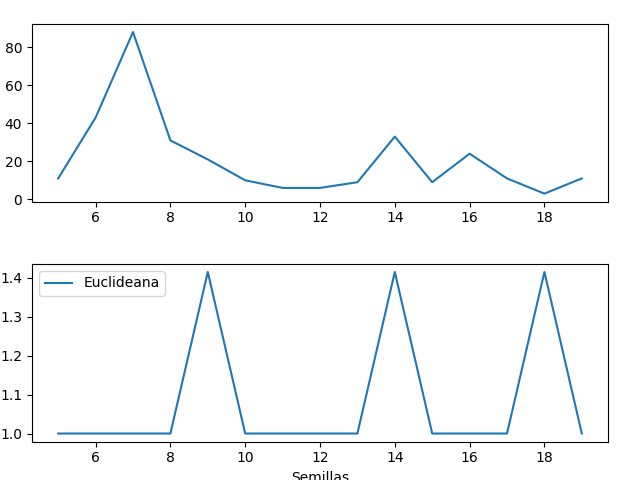
\includegraphics[width=\linewidth]{80x80-5-20.png}
           \caption{80x80}
           \label{fig:westminster_aerea}
        \end{subfigure}
        \caption{Variacion en semillas de 5-20}
        \label{f3}
\end{figure}

En la figura \ref{f3} se observa la misma variaci\'on en los tama\~nos pero en esta ocasi\'on tomando un numero de semillas de 5-20, as\'i mismo comparando tanto la distancia euclideana como la manhatthan. Aqu\'i ya se observa que es m\'as variable la distancia m\'axima seg\'un el n\'umero de semillas que se utiliza. 

\begin{figure}[H]
       \centering
       \begin{subfigure}[b]{0.45\linewidth}
           
\includegraphics[width=\linewidth]{14treintaveinte_14.png}
           \caption{30x30}
           \label{fig:westminster_lateral}
        \end{subfigure}
        \begin{subfigure}[b]{0.45\linewidth}
            
\includegraphics[width=\linewidth]{14cincuentaveinte_14.png}
            \caption{50x50}
            \label{fig:westminster_aerea}
        \end{subfigure}
 \begin{subfigure}[b]{0.45\linewidth}
            
\includegraphics[width=\linewidth]{14ochentaveinte_14.png}
            \caption{80x80}
            \label{fig:westminster_aerea}
        \end{subfigure}
        \caption{Grieta en celdas de 3 y 5 semillas.}
        \label{f4}
\end{figure}

En la figura \ref{f4} se observa una variaci\'on del tama\~no de la grieta en celdas de 30,50 y 80 cuando tenemos 14 semillas.

\begin{figure}[H]
  \begin{center}
    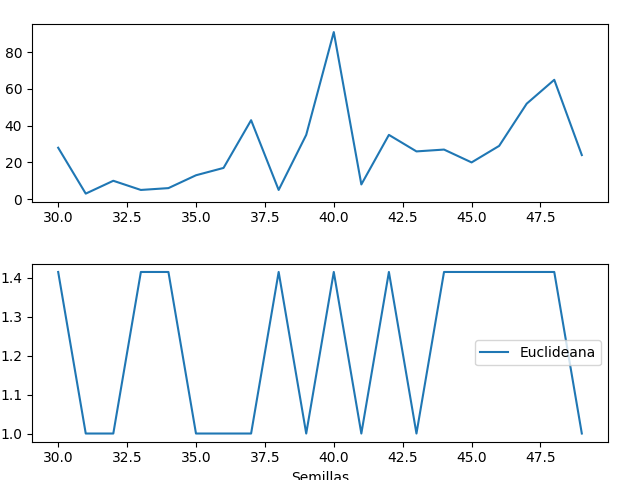
\includegraphics[width=10cm]{80x80-30-50.png}
  \end{center}
  \caption{Semillas de 30-50.}
  \label{f5}
\end{figure}

Finalmente, para fines ilustrativos se realiz\'o una variaci\'on en el n\'umero de semillas la cual se muestra en la figura \ref{f5} tomando una cantidad de 30-50 con un tama\~no de la  celda de 80x80.
El resto de las im\'agenes generadas se encuentran en el repositorio \citep{ana}. De igual manera en el repositorio se adjuntan gifs donde se puede observar mejor como va cambiando la grieta conforme aumenta n\'umero de semillas en tama\~nos de 30x30,50x50 y80x80.

  \section{Conclusi\'{o}n.}\label{con}
Cuando tenemos un menor tama\~no en las celdas es m\'as fac\'il que la grieta que se genera fracture la pieza as\'i mismo la distancia m\'axima euclideana es mayor conforme disminuye el tama\~no de la celda, a comparaci\'on de la distancia manhatthan que aumenta con el tama\~no de la celda,la distancia euclideana no va necesariamente en funci\'on del n\'umero de semillas,sino m\'as bien del tama\~no de la celda.

  \bibliography{P4}
  \bibliographystyle{plainnat}
\end{document}